\documentclass[aspectratio=169,notes]{beamer}

\usepackage{pgfpages}

% Allows including images
\usepackage{graphicx} 

% ???
\usepackage[english]{babel}

%\setbeameroption{show notes on second screen}
%\setbeameroption{hide notes}

% Use metropolis theme
\usetheme[
	outer/progressbar=foot,
	outer/numbering=counter,
	%titleformat=allsmallcaps
	]{metropolis} 
\definecolor{blue}{HTML}{056466}
\definecolor{white}{HTML}{FFFFFF}

 % Sans Serif Font
%\usepackage[semibold,oldstyle]{sourcesanspro}

 % The command \nth{<number>} generates English ordinal numbers of the form 1st, 2nd, 3rd, 4th
%\usepackage[super]{nth}

% Theme colors are derived from these two elements
\setbeamercolor{alerted text}{fg=blue}
\setbeamercolor{frametitle}{bg=blue}
\setbeamercolor{normal text}{bg=white}

% Set EBI logo footer
%  \setbeamertemplate{footline}{%
%         \includegraphics[height=1cm]{img/EBI_logo.png}%
% 		%\hfill%
% 		% \insertsectionnavigationhorizontal{.5\textwidth}{}{}
% }


\title{Statistical methods for data integration}
\author{Ricard Argelaguet \\ \textit{ricard@ebi.ac.uk}}
\institute{European Bioinformatics Institute (EMBL-EBI) \\ University of Cambridge}
%\date{\today}


%  (SI) units 
\usepackage{siunitx}

% bibliography
% \usepackage[style=authoryear, backend=biber, sortlocale=en_US, natbib=false, url=false, doi=true, eprint=false]{biblatex}
% \usepackage[style=authoryear,,backend=bibtex]{biblatex}
\usepackage[hyperref=true, url=false, backref=false, backend=biber, style=authoryear, giveninits=true]{biblatex}
\addbibresource{references/bibliography.bib}
\renewcommand*{\bibfont}{\tiny}

% \renewbibmacro*{cite}{
%   \iffieldundef{shorthand}
%     {\ifthenelse{\ifnameundef{labelname}\OR\iffieldundef{labelyear}}
%        {\usebibmacro{cite:label}
%         \setunit{\printdelim{nonameyeardelim}}}
%        {\printnames{labelname}
%         \setunit{\printdelim{nameyeardelim}}}
%      \usebibmacro{cite:labeldate+extradate}
%      \setunit{\addcomma\space}
%      \usebibmacro{journal}}
%     {\usebibmacro{cite:shorthand}}
% }

\DeclareCiteCommand{\footcite}[\mkbibfootnote]
  {\usebibmacro{prenote}}
  {\printnames{author}
   \printfield{title}{}
   \printfield{journaltitle}{}
   \printfield{year}}
  {\addsemicolon\space}
 {\usebibmacro{postnote}}
  \newcommand\footnotenonum[1]{
  \begingroup
  \renewcommand\thefootnote{}\footnote{#1}
  \addtocounter{footnote}{-1}
  \endgroup
}

%\setbeamerfont{footnote}{size=\footnotesize}
\setbeamerfont{footnote}{size=\tiny}

% Foot note without markers
\newcommand\blfootnote[1]{%
  \begingroup
  \renewcommand\thefootnote{}\footnote{#1}%
  \addtocounter{footnote}{-1}%
  \endgroup
}

% Remove indent in the footnotes
\addtobeamertemplate{footnote}{\hskip -1em}{}


%%%%%%%%%%%%%%%%%%%%%%%%%%%%%%%%%%%%%%%%%%%%%%%%%%%%%%%%%%%%%%%%%%%%
%
%  File: utils.tex
%
%  Utilities for typesetting in latex
%
%
%
%%%%%%%%%%%%%%%%%%%%%%%%%%%%%%%%%%%%%%%%%%%%%%%%%%%%%%%%%%%%%%%%%%%%

%Help:
%- Difference between boldsymbol, boldmath, bm, mathbf ??
%- Differnece betwen \def and \newcommand: \def is a tex primitive, \newcommand is a LaTeX overlay on top of \def. Advantages: checks whether commanda lready exists, allows you to define optional arguments.
% \ensuremath?: around math components in every macro that I define use mathrm for default non-italic letters

%% Math abbreviations %%

\newcommand{\beq}{\begin{equation*}}
\newcommand{\eeq}{\end{equation*}}

\newcommand{\baln}{\begin{align*}}
\newcommand{\ealn}{\end{align*}}
\def\baln#1\ealn{\begin{align*}#1\end{align*}}

\newcommand{\bmat}{\begin{bmatrix}}
\newcommand{\emat}{\end{bmatrix}}
%\def\bmat#1\emat{\begin{bmatrix}#1\end{bmatrix}}

% For commenting:
%\newcommand{\comment}[1]{\textsl{\textcolor{Gray}{#1}}}
%\newcommand{\fixme}[1]{\textsl{\textcolor{Gray}{Fixme: #1}}}

%MathBold-Font
%\newcommand{\mbf}[1]{{\ensuremath{\mathbf{#1}}}}

%Standard commands used throughout the thesis
%\newcommand{\data}{\mathcal{D}}
%\newcommand{\model}{\mathcal{H}}
%\newcommand{\GPM}{\mathcal{H}_{\text{GP}}}
%\newcommand{\datatest}{\mathcal{D}_{\text{test}}}
%\newcommand{\pl}{\ensuremath{p_{\textnormal{L}}}}
%\newcommand{\TK}{\ensuremath{\bTheta_{\textnormal{K}}}}
%\newcommand{\hTL}{\ensuremath{\hat{\btheta}_{\textnormal{L}}}}
%\newcommand{\hTK}{\ensuremath{\hat{\bTheta}_{\textnormal{K}}}}
%\newcommand{\TL}{\ensuremath{\btheta_{\textnormal{L}}}}
%\newcommand{\TT}{\ensuremath{\btheta}}
%\newcommand{\x}{\ensuremath{\bfx}}
%\newcommand{\X}{\ensuremath{\bfX}}

%\newcommand{\rmd}{\mathrm{d}}

%% Sets of numbers (real, natural, complex) etc. %%

%\newcommand{\R}{{\sf R\hspace*{-0.9ex}\rule{0.15ex} {1.5ex}\hspace*{0.9ex}}}
\newcommand{\R}{\ensuremath{\mathbb{R}}}
\newcommand{\N}{{\sf N\hspace*{-1.0ex}\rule{0.15ex}{1.3ex}\hspace*{1.0ex}}}
%\newcommand{\C}{{\sf C\hspace*{-0.9ex}\rule{0.15ex}{1.3ex}\hspace*{0.9ex}}}

% constant
\newcommand{\const}{{\rm const.}}

% argmin and argmax
\DeclareMathOperator*{\argmin}{arg\,min}
\DeclareMathOperator*{\argmax}{arg\,max}
%\newcommand{\argmax}{\operatornamewithlimits{argmax}}

%% Commonly used line/arrow symbols %%
\newcommand{\indep}{\bot \hspace{-0.6em} \bot}  % orthogonal/independent variables
\newcommand{\arrow}{\rightarrow}
\newcommand{\given}{\,|\,}
\newcommand{\twolines}{\,||\,}
\newcommand{\narroweq}{\!\!=\!\!}


%% Authors %%
%\newcommand{\TODO}[1]{{\color{red}\fbox{TODO} #1}}
%\newcommand{\OLI}[1]{{\color{blue}\fbox{OLI} #1}}
%\newcommand{\FLO}[1]{{\color{green}\fbox{FLO} #1}}
%\newcommand{\RIC}[1]{{\color{orange}\fbox{CL} #1}}
%\newcommand{\new}[1]{{\color{magenta}#1}}
%\newcommand{\old}[1]{{\color[rgb]{0.4,0.6,0.4}#1}}

%% Distributions %%
\newcommand{\Ndist}[2]{\mathcal{N}\left(#1 \given #2\right)} % normal(x|mean,variance)
\newcommand{\Gdist}[2]{\mathcal{G}\left(#1 \given #2\right)} % gamma(x|a,b)
\newcommand{\Udist}[2]{\mathcal{U}\left(#1 \given #2\right)} % uniform(x|min,max)
\newcommand{\Wdist}[2]{\mathcal{W}\left(#1 \given #2\right)} % wishart(x|v,K)
\newcommand{\Bdist}[2]{\text{Beta}\left(#1 \given #2\right)} % bernoulli(x|theta)
%\newcommand{\Bdist}[2]{\mathcal{B}\left(#1 \given #2\right)} % binomial(x|N,theta)
%\newcommand{\Uniformdist}{\mathbb{U}}
%\newcommand{\Bernoulli}{\mathcal{B}}
%\newcommand{\Binomial}{\mathcal{B}}
%\newcommand{\Normal}{\mathcal{N}} %\gamma{x}{0,1}.
%\newcommand{\simnormal}[3]{#1\sim\mathcal{N}(#2 \;,\; #3)}   %\Normal{x}{0,1}.
%\newcommand{\Normal}[3]{\normal{#1}{\;#2\;,\;#3}}
%\newcommand{\sige}{\sigma^2_{\mathrm{e}}}
%\newcommand{\sigg}{\sigma^2_{\mathrm{g}}}
%\newcommand{\hatsige}{\hat\sigma^2_{\mathrm{e}}}
%\newcommand{\hatsigg}{\hat\sigma^2_{\mathrm{g}}}

% Parents and children
%\newcommand{\pa}[1]{{\rm pa_\mathit{#1}}}
%\newcommand{\cp}[2]{{\rm cp_\mathit{#1}^{(\mathit{#2})}}}
%\newcommand{\ch}[1]{{\rm ch_\mathit{#1}}}

% Neighbours
%\newcommand{\neigh}[1]{{\rm ne_\mathit{#1}}}

% KL divergence
\newcommand{\KL}{{\rm KL}}

% Variance and Covariance
\newcommand{\var}{{\rm Var}}
\newcommand{\cov}{{\rm Cov}}

% Entropy
\newcommand{\entropy}{{\mathbb{H}}}

\newcommand{\Tau}{\mathrm{T}}

\newcommand{\cip}{\mbox{$\perp\!\!\!\perp$}}
\newcommand{\condindep}[3]{#1~\cip~#2~|~#3}
\newcommand{\nocondindep}[3]{#1~\mbox{$\not\!\perp\!\!\!\perp$}~#2~|~#3}
\newcommand{\dir}[2]{{\rm Dir}(#1|#2)}

\newcommand{\Lagr}{\mathcal{L}}
\newcommand{\bTau}{\mbox{\boldmath $\Tau$}}
\newcommand{\bDelta}{\mbox{\boldmath $\Delta$}}
\newcommand{\bbeta}{\mbox{\boldmath $\beta$}}
\newcommand{\bmu}{\mbox{\boldmath $\mu$}}
\newcommand{\bnu}{\mbox{\boldmath $\nu$}}
\newcommand{\balpha}{\mbox{\boldmath $\alpha$}}
\newcommand{\bepsilon}{\mbox{\boldmath $\epsilon$}}
\newcommand{\bgamma}{\mbox{\boldmath $\gamma$}}
\newcommand{\bvarsigma}{\mbox{\boldmath $\varsigma$}}
\newcommand{\bsigma}{\mbox{\boldmath $\sigma$}}
\newcommand{\bSigma}{\mbox{\boldmath $\Sigma$}}
\newcommand{\btau}{\mbox{\boldmath $\tau$}}
\newcommand{\blambda}{\mbox{\boldmath $\lambda$}}
\newcommand{\bLambda}{\mbox{\boldmath $\Lambda$}}
\newcommand{\bpi}{\mbox{\boldmath $\pi$}}
\newcommand{\bpsi}{\mbox{\boldmath $\psi$}}
\newcommand{\bchi}{\mbox{\boldmath $\chi$}}
\newcommand{\bxi}{\mbox{\boldmath $\xi$}}
\newcommand{\bXi}{\mbox{\boldmath $\Xi$}}
\newcommand{\bPsi}{\mbox{\boldmath $\Psi$}}
\newcommand{\bphi}{\mbox{\boldmath $\phi$}}
\newcommand{\bPhi}{\mbox{\boldmath $\Phi$}}
\newcommand{\bZeta}{\mbox{\boldmath $\zeta$}}

\newcommand{\btheta}{\mbox{\boldmath $\theta$}}
\newcommand{\bTheta}{\mbox{\boldmath $\Theta$}}
\newcommand{\bOmega}{\mbox{\boldmath $\Omega$}}

\newcommand{\Bmath}[1]{\mbox{\boldmath $#1$}}

%\newcommand{\fastfig}[4]{
%\begin{center}
%\begin{figure}[htb!]
%\centerline{\epsfig{figure=#1,width=#2}}
%\caption[short]{#3}
%\label{#4}
%\end{figure}
%\end{center}
%}

\newcommand{\I}{{\bf I}}
\newcommand{\boldzero}{{\bf 0}}
\newcommand{\boldone}{{\bf 1}}

\newcommand{\bfa}{{\bf a}}
\newcommand{\bfb}{{\bf b}}
\newcommand{\bfc}{{\bf c}}
\newcommand{\bfd}{{\bf d}}
\newcommand{\bfe}{{\bf e}}
\newcommand{\bff}{{\bf f}}
\newcommand{\bfg}{{\bf g}}
\newcommand{\bfh}{{\bf h}}
\newcommand{\bfi}{{\bf i}}
\newcommand{\bfk}{{\bf k}}
\newcommand{\bfl}{{\bf l}}
\newcommand{\bfm}{{\bf m}}
\newcommand{\bfp}{{\bf p}}
\newcommand{\bfr}{{\bf r}}
\newcommand{\bfs}{{\bf s}}
\newcommand{\bft}{{\bf t}}
\newcommand{\bfu}{{\bf u}}
\newcommand{\bfv}{{\bf v}}
\newcommand{\bfw}{{\bf w}}
\newcommand{\bfx}{{\bf x}}
\newcommand{\bfy}{{\bf y}}
\newcommand{\bfz}{{\bf z}}

\newcommand{\E}{\mathbb{E}}
\newcommand{\bfA}{{\bf A}}
\newcommand{\bfB}{{\bf B}}
\newcommand{\bfC}{{\bf C}}
\newcommand{\bfD}{{\bf D}}
\newcommand{\bfE}{{\bf E}}
\newcommand{\bfF}{{\bf F}}
\newcommand{\bfG}{{\bf G}}
\newcommand{\bfH}{{\bf H}}
\newcommand{\bfI}{{\bf I}}
\newcommand{\bfJ}{{\bf J}}
\newcommand{\bfK}{{\bf K}}
\newcommand{\bfL}{{\bf L}}
\newcommand{\bfM}{{\bf M}}
\newcommand{\bfQ}{{\bf Q}}
\newcommand{\bfR}{{\bf R}}
\newcommand{\bfS}{{\bf S}}
\newcommand{\bfT}{{\bf T}}
\newcommand{\bfU}{{\bf U}}
\newcommand{\bfV}{{\bf V}}
\newcommand{\bfW}{{\bf W}}
\newcommand{\bfX}{{\bf X}}
\newcommand{\bfY}{{\bf Y}}
\newcommand{\bfZ}{{\bf Z}}
\newcommand{\llangle}{{\langle \hspace{-0.7mm} \langle}}
\newcommand{\rrangle}{{\rangle \hspace{-0.7mm} \rangle}}
\newcommand{\define}{\stackrel{\mathrm{def}}{=}}

\newcommand{\la}{\langle}
\newcommand{\ra}{\rangle}
\newcommand{\La}{\left\langle}
\newcommand{\Ra}{\right\rangle}
%\newcommand{\EXP}[1]{\left\langle #1 \right\rangle}
%\newcommand{\vectwo}[2]{\left[\begin{array}{c} #1 \\ #2 \end{array}\right]}
%\newcommand{\vecn}[1]{\left[\begin{array}{c} #1 \end{array}\right]}
%\newcommand{\half}{{\scriptstyle \frac{1}{2}}}
%\newcommand{\col}{\mathrm{vec}}

%\newcommand{\trans}[1]{{#1}^{\ensuremath{\mathsf{T}}}}
%\newcommand{\T}{{\rm T}}
\newcommand{\diag}{{\rm diag}}
%\newcommand{\exp}{\mathcal{exp}}
\newcommand{\Tr}{\mbox{Tr}}
\newcommand{\tr}{\mbox{tr}}
%\newcommand{\diff}[1]{{\,d#1}}
%\newcommand{\vgraph}[1]{
%  \newpage
%  \begin{center}
%  {\large \bf #1}
%  \end{center}
%  \vspace{2mm}
%}

%\newcommand{\high}[1]{\textcolor{blue}{\emph{#1}}}
%\newcommand{\cut}[1]{}
%\newcommand{\citeasnoun}[1]{\citeN{#1}}
%\newcommand{\citemulti}[2]{(#1, \citeyearNP{#2})}
%\newcommand{\citemultiN}[2]{#1 (\citeyearNP{#2})}
%\newcommand{\Sum}{{\displaystyle \sum}}

%%%%%%%%%%%%%%%%%%%%%%%%%%%%%%%%%%%%%%%%%%%%%%%%%%%%%%%%%%%%%%%%%%%%



\begin{document}

 	% Print the title page as the first slide
	\begin{frame}
	\titlepage
	\end{frame}
	
	% \begin{frame}{Overview}
	% \end{frame}

	% \begin{frame}{Why multi-omics?}
	% \centering
	% \includegraphics[height=6cm]{img/Ritchie2015_overview.png}\footcite{Ritchie2015}
	% \end{frame}
	
	\begin{frame}{Why multi-omics?}
	The integrative analysis of diverse data modalities in a systems biology approach will capture better the molecular phenotypic varaition of biological systems\\
	\leavevmode\newline
	\centering
	\includegraphics[height=5.5cm]{img/Sun2016_multiomics.png}
	\end{frame}

	\begin{frame}{Abstraction of a multi-omics experimental design}
	\centering
	\includegraphics[height=5.5cm]{img/matrices.png}
	\end{frame}

	\begin{frame}{Strategies for multi-omics data integration}
	The first step is to choose the anchoring unit for the integration \\
%	\begin{itemize}
%		\item \textbf{Horizontal integration} features as the anchor
%		\item \textbf{Vertical integration} samples as the anchor
%	\end{itemize}	
	\leavevmode\newline
	\centering
	\includegraphics[height=5.5cm]{img/anchor_overview.png}
	\end{frame}

	% \begin{frame}{Strategies for multi-omics data integration in \textit{matched} assays}
	% By having a common sample space, the aim of these methods is to discover and exploit associations within and between molecular layers. Broadly speaking, there are two types of integration strategies:
	% \centering
	% \includegraphics[height=6cm]{img/Ritchie2015_local_vs_global.png}
	% \end{frame}

	\begin{frame}{Strategies for multi-omics data integration}
	Two general strategies for vertical integration (multi-omics data derived from the same set of samples);
	\begin{itemize}
		\item \textbf{Local analysis}: test for marginal associations between features from different molecular layers. Generally supervised.
		\item \textbf{Global analysis}: exploit the dependencies between the features to construct a mathematical representation of the data. Generally unsupervised.
	\end{itemize}	
	\end{frame}

	\begin{frame}{Local analysis}
	The most prominent examples of local analysis are quantitative trait loci mapping (GWAS and eQTLs)\footcite{Ritchie2015}:\\
	\leavevmode\newline
	\centering
	\includegraphics[height=5cm]{img/Ritchie2015_local_analysis.png}
	\blfootnote{eQTL: expression Quantiative Trait Loci}
	\end{frame}

	\begin{frame}{Local analysis}
	Local analysis is typically done using (generalised) linear models\\
	\leavevmode\newline
	\centering
	\includegraphics[height=5.5cm]{img/gwas_eqtl.png}
	\blfootnote{GWAS: Genome-Wide Association Study (GWAS)\\eQTL: expression Quantiative Trait Loci}
	\end{frame}

	\begin{frame}{Local analysis}
	\leavevmode\newline
	\centering
	\includegraphics[height=6cm]{img/linear-regression.png}
	\end{frame}



	\begin{frame}{Global analysis}
	In global analysis the aim is to exploit the relationship between all features to create useful mathematical representations\footcite{Ritchie2015}\\
	\leavevmode\newline
	\centering
	\includegraphics[height=4.5cm]{img/Ritchie2015_global_analysis.png}
	\end{frame}

	\begin{frame}{Global analysis}
	Challenges in (global) multi-omics data integration:
	\begin{itemize}
		\item Data collected using different techniques (i.e. data modalities) generally exhibit heterogeneous statistical properties
		\item Large amounts (and different patterns) of missing values
		\item Overfitting
		\item Undesired sources of heterogeneity
		\item Complexity of the data requires unsupervised interpretable approaches
	\end{itemize}
	\end{frame}

	\begin{frame}{Latent variable models}
	Given a dataset $\mathbf{Y}$ of $N$ samples and $D$ features, latent variable models exploit the dependencies between the features to reduce the dimensionality of the data. The mapping from the high-dimensional to the low-dimensional space is performed via a function $f(\bfY|\bTheta)$:\\
	\leavevmode\newline
	\centering
	\includegraphics[height=4cm]{img/latent_variable_models.png}
	\end{frame}

	\begin{frame}{Principal component analysis (PCA)}
	Principal Component Analysis (PCA) is the most popular technique for dimensionality reduction.\\
	\leavevmode\newline
	\centering
	
\includegraphics[height=4.75cm]{img/pca.jpeg}\\
  	\tiny Credit to Raunak Joshi \par
	\end{frame}


	\begin{frame}{Principal component analysis (PCA)}
	PCA defines $f(\bfY|\bTheta)$ to be a linear transformation via a matrix $\bfW \in \R^{D \times K}$ that maps the observations $\bfY \in \R^{N \times D}$ onto the latent space $\bfZ \in \R^{N \times K}$.\\
	\leavevmode\newline
	\centering
	\includegraphics[height=3.5cm]{img/matrix_factorisation.png}
	% \centering
	% 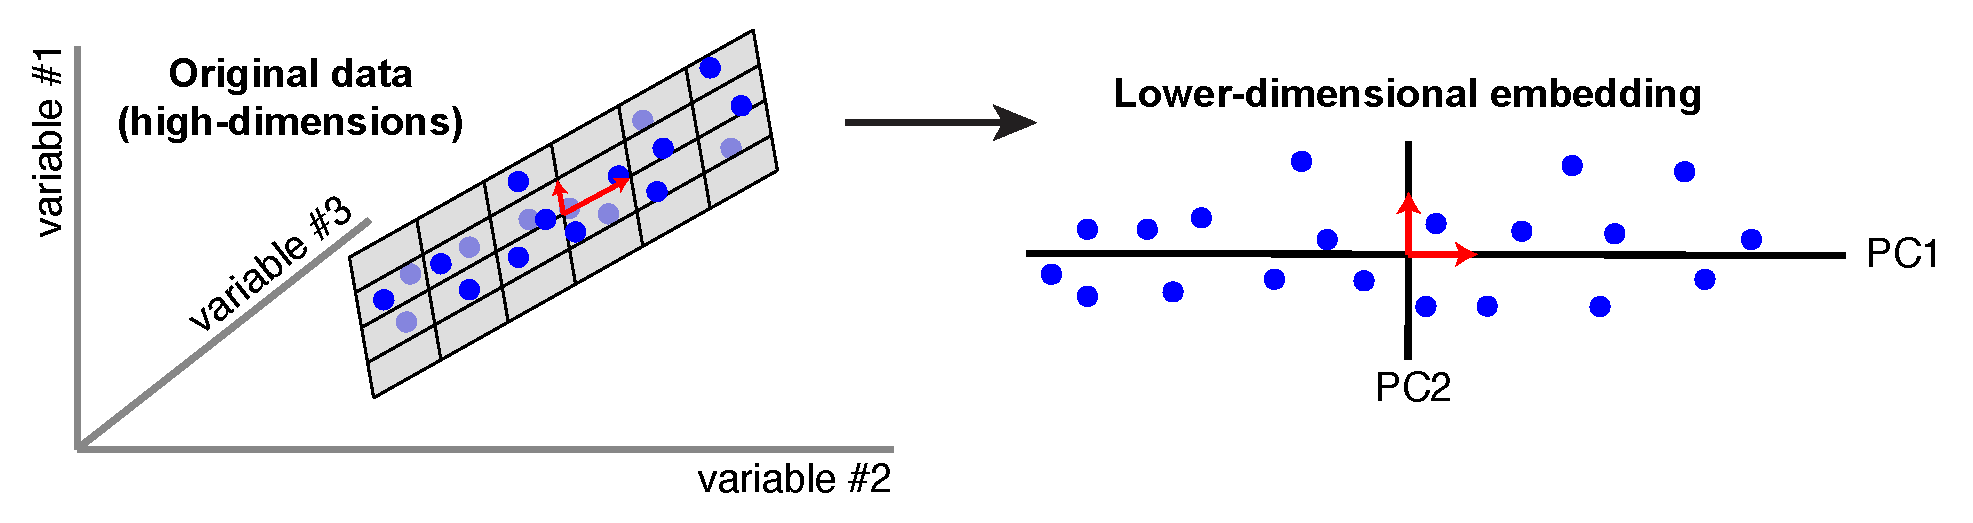
\includegraphics[height=2.8cm]{img/pca_overview.pdf}
	% \[
	% 	\mathbf{Z} = \mathbf{Y}\mathbf{W}
	% \]
	% The matrix  contains the low-dimensional representation for each sample (i.e. the factors).\\
	% The matrix $\bfW \in \R^{D \times K}$ contains the feature weights (i.e. the gene scores)
	\end{frame}

	% \begin{frame}{Principal component analysis (PCA)}
	% \end{frame}

	\begin{frame}{Mathematical derivation of PCA: maximum variance formulation}
	The aim in PCA is to infer the matrix $\bfW$ such that the variance of $\bfZ$ (the projected data) is maximised. If we consider a single latent factor, the variance of the projected data is:
	\begin{align*}
		\sigma^2 &= \frac{1}{N}\sum_{n=1}^{N} (\bfz_n - \hat{\bfz})^{2} \\
				 &= \frac{1}{N}\sum_{n=1}^{N} (\bfy_n^T \bfw - \hat{\bfy}^T\bfw)^{2}
	\end{align*}
	where $\hat{\bfy}$ is a vector with the feature-wise means. If we center the data this simplifies to:
	\begin{equation*}
		\sigma^2 = \frac{1}{N}\sum_{n=1}^{N} (\bfy_n^T \bfw)^{2}
	\end{equation*}
	\end{frame}

	\begin{frame}{Mathematical derivation of PCA: maximum variance formulation}
	A bit of algebra allows us to define this equation in terms of the (centered) data covariance matrix: $\bfS = \frac{1}{N}\sum_{n=1}^{N} \bfy_n\bfy_n^T$:
	\begin{align*}
		\sigma^2 &= \frac{1}{N}\sum_{n=1}^{N} (\bfy_n^T \bfw)^T (\bfy_n^T \bfw) \\
		=& (\bfw^T \bfy_n) (\bfy_n^T \bfw) \\
		=& \bfw^T (\bfy_n \bfy_n^T) \bfw \\
		=& \bfw^T \bfS \bfw
	\end{align*}
	\end{frame}

	\begin{frame}{Mathematical derivation of PCA: maximum variance formulation}
	The optimisation problem to find the first latent variable could be defined as:
	\[
		\hat{\bfw} = \argmax_{\bfw} \bfw^T \bfS \bfw
	\]
	% where we have removed any term that is constant and does not affect the optimisation.\\
	\leavevmode\newline
	\textbf{(Q) Maximising this expression does not work, we need a constrain. Why?}
	% (Solution) The weights need to be constraint to have a constant norm (one, arbritrarily), otherwise maximizing the expression above would simply lead to the weight vector having infinite norm, as this leads to an infinite variance.
	\end{frame}

	\begin{frame}{Mathematical derivation of PCA: maximum variance formulation}
	The constrained optimisation problem can be defined as:
	\[
		\hat{\bfw} = \argmax_{\|\bfw\|=1} \bfw^T \bfS \bfw
	\]
	It can be solved by introducing a Lagrange multiplier $\lambda$ to enforce the constraint:
	\[
		f(\bfW,\lambda) = \bfw^T \bfS \bfw + \lambda (1-\bfw^T\bfw)
	\]
	By setting the derivative $\frac{\partial f(\bfW,\lambda)}{\partial \bfw}$ to zero, we obtain the following equation:
	\[
		\bfS \bfw = \lambda \bfw
	\]
	which should be familiar (perhaps in this form $\bfA \bfv = \lambda \bfv$)?
	\end{frame}

	\begin{frame}{Mathematical derivation of PCA: maximum variance formulation}
	Among all possible orthonormal basis, the one that maximises the projected variance corresponds to the basis defined by the eigenvectors of the covariance matrix $\bfS$. These vector basis are called the principal components.\\
	\leavevmode\newline
	The corresponding eigenvalue $\lambda$ corresponds to the variance $\sigma$ (proof in the appendix).
	% \leavevmode\newline
	% To obtain the low-dimensional representation of the data we just need to multiply each data point $\bfy_n$ by $\bfw$:
	% \[
	% 	z_n = \bfy_n^T \bfw 
	% \]
	\end{frame}

	% \begin{frame}{Mathematical derivation of PCA: maximum variance formulation}
	% The eigenvalue $\lambda$ corresponds to the variance $\sigma$. The proof requires knowing the following equality $Var(X) = \E[X^2] - (\E[X])^2$

	% some algebra:
	% \begin{align}
	% \sigma^2 = Var($\bfz$) &= \E[\bfz^T\bfz] - (\E[\bfz])^2 \\
	% &= \E[(\bfY\bfw)^T (\bfY\bfw)] - (\E[\bfY \bfw])^2 \\
	% % &= \E[(\bfy^T\bfw)(\bfy^T\bfw)] - (\bfw \E[\bfy^T])^2 \\
	% \end{align}
	% If we assume that the data is centered then $\E[\bfy^T]=0$, so the second term disappears.
	% \[
	% \sigma^2 = \E[\bfw \bfY^T \bfT \bfw]
	% \]
	% where the term $\bfY^T \bfY$ corresponds to the covariance matrix $\bfS$. Therefore:
	% \[
	% \sigma^2 = \E[\bfw \bfS \bfw] = 
	% \]
	% \end{frame}

	% \sigma^2 = \frac{1}{N}\sum_{n=1}^{N} (\bfz_n - \hat{\bfz})^{2} = \frac{1}{N}\sum_{n=1}^{N} (\bfy_n \bfw - \hat{\bfy}\bfw)^{2}


	\begin{frame}{Generalisation to multiple principal components}
	Most data can not be well-described by a single principal component. The $k$-th principal component can be found by subtracting from $\bfY$ the reconstructed data by the previous $k-1$ principal components: 
	%If we define $\bfz_k=\bfY \bfw_k $ to be the $k$-th principal component:
	\[
		\hat{\bfY} = \bfY - \sum_{k=1}^{K} (\bfz_k \bfw_k^T)
	\]
	and repeating the procedure above using the reconstructed covariance matrix $\hat{\bfS}$ as input
	% \[
	% 	\hat{\bfw_k} = \argmax_{\|\bfw_k\|=1} \bfw_{k}^{T} \hat{\bfS_k} \bfw_k
	% \]
	% \centering
	% \includegraphics[height=3cm]{img/pca_reconstruction.png}
	% \blfootnote{Figure by Alex Williams} %http://alexhwilliams.info/itsneuronalblog/2016/03/27/pca/
	\end{frame}

	\begin{frame}{Finding the \textit{right} number of Principal Components}
	Principal components are ranked by the amount of variance they capture in the original dataset, a scree plot can provide some sense of how many components are needed.\\
	\leavevmode\newline
	\centering
	\includegraphics[height=4cm]{img/scree_plot.png}
	%\blfootnote{Figure by Alex Williams} %http://alexhwilliams.info/itsneuronalblog/2016/03/27/pca/
	\end{frame}

	\begin{frame}{Problems of using PCA for multi-omics data integration}
	PCA is a great exploratory tool for single multivariate data sets, but it has important pitfalls in the analysis of multi-omics data:
	\begin{itemize}
		\item Does not generalise to an arbitrary number of data modalities.
		\item No natural way to combine different data modalities (binary data with continuous data).
		\item Cannot handle missing values.
	\end{itemize}
	\end{frame}


	\begin{frame}{Canonical correlation analysis}
	Canonical Correlation Analysis (CCA) is a simple extension of PCA to find linear components that capture correlations between \textbf{two} datasets \footcite{Hotteling1936}.\\
	\leavevmode\newline
	Given two data matrices $\bfY_1 \in \R^{N \times D_1}$ and $\bfY_2 \in \R^{N \times D_2}$ CCA finds a set of linear combinations $\bfU \in \R^{D_1 \times K}$ and $\bfV \in \R^{D_2 \times K}$ with maximal cross-correlation.\\ 
	\leavevmode\newline
	For the first pair of canonical variables, the optimisation problem is:
	\[
		(\hat{\bfu_1}, \hat{\bfv_1}) = \argmax_{\|\bfu_1\|=1,\|\bfv_1\|=1} corr(\bfu_{1}^T \bfY_1, \bfv_{1}^T \bfY_2)
	\]
	%As in PCA, the linear components are constraint to be orthonormal. 
	%Hence, the first pair of canonical variables $\bfu_1$ and $\bfv_1$ contain the linear combination of variables that have maximal correlation. Subsequently, Therefore, the second pair of canonical variables $\bfu_2$ and $\bfv_2$ is found out of the residuals of the first canonical variables.\\
	% (Q) What are the limitation of CCA?
	\end{frame}

%	\begin{frame}[allowframebreaks]{References}
%  	\printbibliography[heading=none]
%	\end{frame}

\end{document}
